\section{A network understood completely, and what comes next}
\label{sec:modadd}

\begin{sessioncard}
\textbf{Session 8.} \emph{Goal:} see one network whose algorithm is known completely, learn what its training
looks like from the inside, and collect the lessons of the seminar.
\emph{Experiments:} we train a small transformer on addition modulo 113 and watch it generalise long after it has
memorised (\cref{exp:grokking}), find the algorithm in its weights (\cref{exp:fourier,exp:modaddlogits}), and
follow the algorithm while it forms (\cref{exp:progress}).
\emph{Prerequisites:} session 2. The session uses the addition theorems for sine and cosine.
\end{sessioncard}

The circuits of session 7 explain a part of what GPT-2 small does on a narrow task. For one family of small
networks the reverse engineering has been carried to the end. The example is due to
\citet{nanda2023progress}, and it is small enough that we can repeat it from scratch.

\subsection{A network that learns late}

The task is addition modulo $P=113$. The input is the sequence $a$, $b$, \tok{=} with
$a,b\in\{0,\dots,P-1\}$, where each number is one token, and the correct output is the number
$c\in\{0,\dots,P-1\}$ with $c\equiv a+b \pmod P$. The model is a transformer with a single layer: four attention
heads, one MLP with $512$ neurons, a stream of width $128$, no $\LN$.

\begin{experiment}[Memorising first, generalising later]\label{exp:grokking} \script{exp\_modadd.py}
There are $113^2=12{,}769$ pairs $(a,b)$. We train on a random $30\%$ of them and test on the rest
(\cref{fig:grokking}, left). Each step of training uses all training pairs. The optimiser is AdamW, a variant
of gradient descent that adapts the step size of every weight, with learning rate $10^{-3}$ and \emph{weight
decay} $1$. Weight decay means that every step also shrinks each weight by a small fraction of its value, so
that weights which the loss does not hold in place drift towards zero. After $1000$ steps the loss on the
training pairs is below $10^{-5}$: the network knows them by heart. On the held-out pairs it is right in $4\%$ of the cases, and its loss there is
far above that of a uniform guess. For thousands of steps nothing seems to happen. Then the test accuracy rises
from $18\%$ at step $4000$ to $68\%$ at step $5000$ and $99\%$ at step $5700$, and soon after the network is
right on every pair. This delayed generalisation is called \emph{grokking} \citep{power2022grokking}.
\end{experiment}

\begin{figure}[t]
\centering
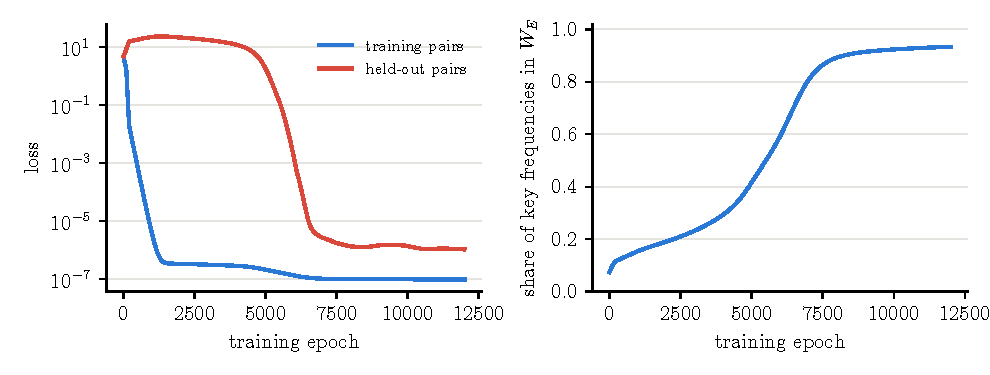
\includegraphics[width=0.95\textwidth]{figures/fig_grokking.pdf}
\caption{Training a one-layer transformer on addition modulo 113. Left: loss on the training pairs and on the
held-out pairs (\cref{exp:grokking}). Right: share of the squared norm of the embedding matrix that lies in the
four frequencies which the final network uses (\cref{exp:progress}).}
\label{fig:grokking}
\end{figure}

What has the network learned when it finally generalises? We might expect something like a table of sums. It
is something else.

\subsection{Finding the algorithm}

\begin{experiment}[The embedding is periodic]\label{exp:fourier} \script{exp\_modadd.py}
The embedding assigns a vector $W_E[a]\in\R^{128}$ to each number $a$. We regard each coordinate of the
embedding as a function of $a$ and decompose it into the functions $\cos(2\pi ra/P)$ and $\sin(2\pi ra/P)$ for
the frequencies $r=1,\dots,56$, which together with the constant function form an orthogonal basis.
\Cref{fig:fourier} shows how much of the squared norm of $W_E$ belongs to each frequency. Four frequencies,
$r=5,7,36,49$, carry $93\%$ of it. The other $52$ frequencies share the remaining $7\%$, of which $4\%$ lies in the single
frequency $r=15$. The network represents a number $a$ by where it lies on four circles: it stores $\cos(2\pi ra/P)$ and $\sin(2\pi ra/P)$ for four values of $r$.
\end{experiment}

\begin{figure}[t]
\centering
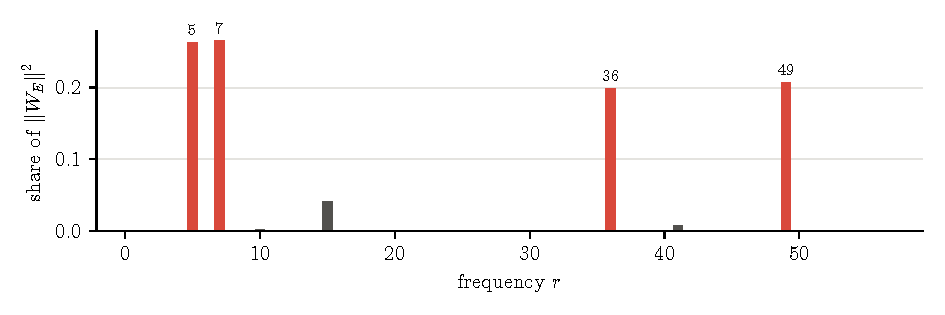
\includegraphics[width=0.9\textwidth]{figures/fig_fourier.pdf}
\caption{Share of the squared norm of the embedding matrix of the trained network that belongs to each
frequency (\cref{exp:fourier}).}
\label{fig:fourier}
\end{figure}

Following this lead through the network, \citet{nanda2023progress} found that it computes as follows, for each of
its frequencies $r$.
\begin{enumerate}
\item The embedding maps the input $a$ to $\cos(2\pi ra/P)$ and $\sin(2\pi ra/P)$, and likewise for $b$.
\item Attention and MLP multiply these numbers and combine the products, by the addition theorems, into the
cosine and sine of the sum. For the cosine,
\[
\cos\!\Big(\frac{2\pi r(a+b)}{P}\Big)=\cos\!\Big(\frac{2\pi ra}{P}\Big)\cos\!\Big(\frac{2\pi rb}{P}\Big)
-\sin\!\Big(\frac{2\pi ra}{P}\Big)\sin\!\Big(\frac{2\pi rb}{P}\Big).
\]
\item The unembedding multiplies these with $\cos(2\pi rc/P)$ and $\sin(2\pi rc/P)$ for every candidate $c$.
By the addition theorem once more,
\[
\cos\!\Big(\frac{2\pi r(a+b)}{P}\Big)\cos\!\Big(\frac{2\pi rc}{P}\Big)
+\sin\!\Big(\frac{2\pi r(a+b)}{P}\Big)\sin\!\Big(\frac{2\pi rc}{P}\Big)
=\cos\!\Big(\frac{2\pi r(a+b-c)}{P}\Big).
\]
The logit of $c$ is approximately a weighted sum of these terms over the frequencies,
\begin{equation}\label{eq:modadd}
\logit(c)\;\approx\;\sum_{r}\text{weight}_r\cdot\cos\!\Big(\frac{2\pi r\,(a+b-c)}{P}\Big)\qquad\text{with positive weights.}
\end{equation}
\end{enumerate}

Why does \eqref{eq:modadd} single out the correct answer? If $c\equiv a+b$, every cosine equals $1$. For any
other $c$ the cosines of different frequencies point in different directions and largely cancel. With all
frequencies and equal weights the cancellation is exact.

\begin{proposition}[Cosines over all frequencies form an indicator]\label{prop:cos}
Let $P\ge2$ be an integer and let $q$ be an integer. Then
\[
\sum_{r=0}^{P-1}\cos\!\Big(\frac{2\pi rq}{P}\Big)=\begin{cases}P&\text{if $q$ is divisible by $P$,}\\ 0&\text{otherwise.}\end{cases}
\]
\end{proposition}
\begin{proof}
If $q$ is divisible by $P$, every angle $2\pi rq/P$ is a multiple of $2\pi$, every term is $1$ and the sum is
$P$. Now let $q$ not be divisible by $P$. Then $\pi q/P$ is not a multiple of $\pi$, so $\sin(\pi q/P)\ne0$.
We multiply the sum by $2\sin(\pi q/P)$ and use the identity $2\sin\phi\cos\psi=\sin(\psi+\phi)-\sin(\psi-\phi)$
with $\phi=\pi q/P$ and $\psi=2\pi rq/P$.
\begin{align*}
2\sin\!\Big(\frac{\pi q}{P}\Big)\sum_{r=0}^{P-1}\cos\!\Big(\frac{2\pi rq}{P}\Big)
&= \sum_{r=0}^{P-1}\Big[\sin\!\Big(\frac{(2r+1)\pi q}{P}\Big)-\sin\!\Big(\frac{(2r-1)\pi q}{P}\Big)\Big] && \by{by the identity}\\
&= \sin\!\Big(\frac{(2P-1)\pi q}{P}\Big)-\sin\!\Big(\frac{-\pi q}{P}\Big) && \by{telescoping sum}\\
&= \sin\!\Big(2\pi q-\frac{\pi q}{P}\Big)+\sin\!\Big(\frac{\pi q}{P}\Big) && \by{since $\sin$ is odd}\\
&= -\sin\!\Big(\frac{\pi q}{P}\Big)+\sin\!\Big(\frac{\pi q}{P}\Big) && \by{period $2\pi$, $q$ an integer}\\
&= 0. && \by{the two terms cancel}
\end{align*}
Dividing by $2\sin(\pi q/P)\ne0$ gives the claim.
\end{proof}

With $q=a+b-c$, the proposition says that the sum over \emph{all} frequencies is $P$ for the correct $c$ and $0$
for every other $c$. A few frequencies are enough. Since $P$ is prime, $\cos(2\pi rq/P)=1$ with $0<r<P$ forces $q$
to be divisible by $P$, so a sum of cosines with positive weights is largest at the correct answer and strictly
smaller everywhere else.

\begin{experiment}[The logits follow the formula]\label{exp:modaddlogits} \script{exp\_modadd.py}
We test \eqref{eq:modadd} on our network. We compute its logits for all $113^3$ triples $(a,b,c)$, subtract for
each pair $(a,b)$ the mean over $c$, and fit the four weights of \eqref{eq:modadd} for the frequencies
$5,7,36,49$ by least squares. The fit explains $98\%$ of the variance of the logits. \Cref{fig:modaddlogits}
shows the logits averaged over all inputs with the same value of $a+b-c$, together with the fit. The fitted
value is $46.5$ at the correct answer and no more than $27.2$ at any wrong one. A formula with four numbers describes a
network with about $227{,}000$ weights.
\end{experiment}

\begin{figure}[t]
\centering
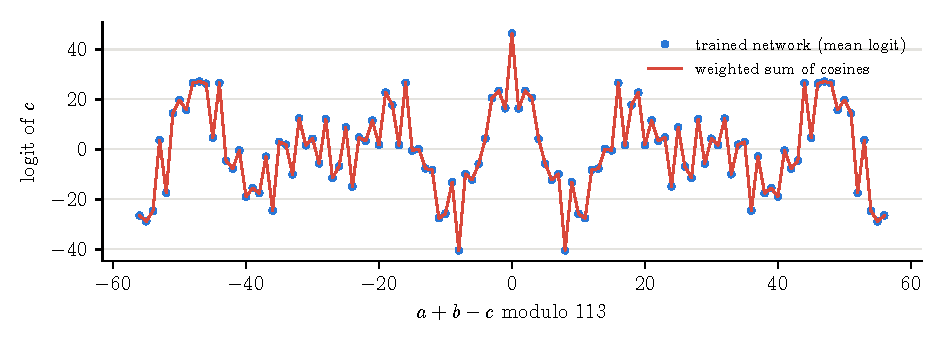
\includegraphics[width=0.9\textwidth]{figures/fig_modadd_logits.pdf}
\caption{Logit of the candidate $c$ in the trained network, averaged over all inputs with the same value of
$a+b-c$, and the fit by a weighted sum of four cosines (\cref{exp:modaddlogits}).}
\label{fig:modaddlogits}
\end{figure}

The network of \citet{nanda2023progress} uses five frequencies, $14,35,41,42$ and $52$, and ours uses four
others. The choice of frequencies depends on the random initialisation, and the algorithm is the same. Other
architectures can learn a different algorithm for the same task \citep{zhong2023clock}.

\subsection{What grokking looks like from the inside}

\begin{experiment}[The algorithm forms gradually]\label{exp:progress} \script{exp\_modadd.py}
Knowing the algorithm, we can measure its presence during training. For every $100$th step we compute the share
of the squared norm of $W_E$ that lies in the four final frequencies (\cref{fig:grokking}, right). At the start
it is $7\%$, the value expected for four frequencies out of $56$. It is $15\%$ at step $1000$, $23\%$ at step
$3000$ and $29\%$ at step $4000$, while the test accuracy is still below $20\%$. It passes $50\%$ when the test
accuracy passes $95\%$, and it keeps rising to $93\%$ long after the test accuracy has reached $100\%$.
\end{experiment}

The curve of the test loss suggests that nothing happens for $4000$ steps and that the network then suddenly
understands. The measurement inside tells a different story. The periodic structure grows from the first steps
on, in a network that still relies on its memorised answers. The test loss falls when the new mechanism has
become strong enough to take over, and the cleaning up continues afterwards. \citet{nanda2023progress} call the
three phases memorisation, circuit formation and cleanup, and they attribute the last one to weight decay,
which favours the solution with smaller weights. A curve that looks like a sudden jump from the outside is a
gradual process on the inside. This is the kind of statement that only an understanding of the mechanism can
deliver.

\subsection{From toy networks to large models}

Can anything like this be done for a large language model? Not completely, and the most developed attempt
combines the tools of sessions 5 to 7. \citet{ameisen2025circuit} replace the MLPs of a model by a relative of
the sparse autoencoder, so that the model is rewritten in terms of latents. For one prompt at a time they then
compute which latents influence which, and they draw the result as an \emph{attribution graph}. The part of the
computation that the latents do not capture is kept in the graph as explicit error terms.
\citet{lindsey2025biology} apply the method to a production model. Two of their findings show what such graphs
can reveal. For a prompt that asks for the capital of the state that contains Dallas, the graph contains latents
for Texas between the input and the answer \tok{Austin}: the model performs the two steps internally. When
writing rhyming verse, the model activates candidate rhyme words at the end of a line \emph{before} it writes
the next line, and then composes the line so that it ends in one of them.

These results are reported from one prompt at a time, with a remainder that is not explained, and in terms of
latents that have all the limits of session 5. The distance between \cref{exp:modaddlogits}, where a formula
accounts for $98\%$ of a network, and the state of the art for large models is the open problem of the field.

\subsection{How not to fool ourselves}
\label{sec:pitfalls}

Interpretability has no ground truth. Nobody can open a language model and look up the right answer, so an
explanation can only be checked against its own predictions. The seminar has met the main ways in which a
result can mislead, each with the control that guards against it.

\begin{center}\small
\begin{tabular}{@{}p{0.27\textwidth}p{0.3\textwidth}p{0.35\textwidth}@{}}
\toprule
Failure & Where we met it & Control \\
\midrule
Decodable is not used. & the probe at the last position (\cref{exp:decodable}) & intervene on the representation \\
\addlinespace
Strong examples flatter. & latent 13484 (\cref{exp:genderlatents}) & test on inputs with known labels, count
how often the unit fires without the concept \\ \addlinespace
The method explains the data and not the model. & autoencoders on random networks (session 5) & the same
analysis on a random model, with shuffled labels, with a random direction \\ \addlinespace
The intervention leaves the range that the model knows. & steering at strength 120 (\cref{exp:steertext}) &
replacement values that occur naturally, a check that unrelated behaviour survives \\ \addlinespace
Compensation hides importance. & head 9.9 (\cref{exp:headpatch}), induction heads (\cref{exp:inductionablate}) &
direct and total effects, ablation of groups \\ \addlinespace
A narrow set of inputs and a good story. & the IOI circuit, our own 12 prompts & state the inputs, predict and
test outside them, report the unexplained remainder \\
\bottomrule
\end{tabular}
\end{center}

A useful habit is to ask of every claim, including our own, which kind of evidence it would need. A claim
that a property is \emph{represented} needs a probe or a latent with a control. A claim that the model
\emph{uses} it needs an intervention with a baseline. A claim that a component \emph{matters} needs patching with
a stated counterfactual. A claim that a circuit \emph{is how the model does it} needs faithfulness,
completeness, minimality and a confirmed prediction on new inputs.

\subsection{After the seminar}

The best next step is to change one of the experiments. Three suggestions, in order of difficulty: replace the
template of the running example by one with other verbs or three names, and see which figures of sessions 2 and
6 survive. Repeat \cref{exp:probe,exp:steer} for another concept, for example whether a sentence is in the past
tense. Train the network of this session on subtraction or multiplication modulo $113$ and find out which of the
steps of the algorithm change.

Four questions are widely seen as open, and the survey of \citet{sharkey2025open} treats them at length. What
are the right units of analysis, given the limits of sparse autoencoders? How can an explanation of open-ended
behaviour be validated? Why do linear representations and superposition emerge, and how much computation fits
into superposition? And what is interpretability good for in practice, for instance for auditing a model
\citep{marks2025auditing}?

\begin{takeaways}
A small transformer that is trained on modular addition first memorises and much later generalises. Its
algorithm can be read from its weights: it represents numbers on a few circles and adds angles, and a formula
with four weights explains $98\%$ of its logits. The algorithm forms gradually during the phase in which the
test loss shows nothing. For large models such complete explanations do not exist. What exists are partial
explanations, and a set of controls that tell a real finding from an artefact.
\end{takeaways}

\subsection*{Questions for the seminar}

\begin{exercise}[Why the modulus is prime]\label{ex:cosprime}
(a) Let $P=112$ and $r=14$. List the integers $q$ with $0<q<P$ for which $\cos(2\pi rq/P)=1$. What would a network
that uses only this frequency know about $a+b$? (b) For a modulus $P$ that is not prime, which frequencies $r$
still have the property that $\cos(2\pi rq/P)=1$ forces $q$ to be divisible by $P$?
\end{exercise}

\begin{exercise}[One frequency is not enough]\label{ex:onefreq}
Suppose that the network used a single frequency $r$ with $0<r<P$, so that the logit of the candidate $c$ is
$\cos(2\pi r(a+b-c)/P)$. (a) Show that some wrong candidate receives the logit $\cos(2\pi/P)$. Hint: since $P$ is
prime, there is an integer $q$ with $rq\equiv1\pmod P$. (b) For $P=113$, compute the margin $1-\cos(2\pi/P)$
between the correct answer and this candidate, using $\cos\phi\approx1-\phi^2/2$ for small $\phi$. (c) Compare
with the margin in \cref{exp:modaddlogits} and explain why the network uses several frequencies.
\end{exercise}

\begin{exercise}[Suddenly understood?]\label{ex:sudden}
A colleague looks at the left panel of \cref{fig:grokking} and says: ``At step 5000 the network suddenly
understood addition.'' (a) Use the right panel to respond. (b) Which measurement would test the
claim that weight decay is responsible for the last phase? (c) What would be the analogue of the right panel for
a large language model, and why is it hard to obtain?
\end{exercise}

\begin{exercise}[A lie detector]\label{ex:critique}
A blog post reports: ``We trained a linear probe on layer 20 of a chat model and can predict with 99\% accuracy
whether the model is about to lie. We have found the model's lie detector.'' List three experiments that are
missing, and say for each which row of the table of \cref{sec:pitfalls} it addresses.
\end{exercise}

\begin{readinglist}
\item \citet{nanda2023progress}, \emph{ICLR}. The complete analysis of the modular addition network, including
the evidence for each step of the algorithm that we did not reproduce.
\item \citet{zhong2023clock}, \emph{NeurIPS}. Shows that networks can learn a second, different algorithm for the
same task. A warning against assuming that there is one mechanism per task.
\item \citet{mueller2025mib}, \emph{ICML}. A benchmark that compares methods for finding circuits and variables on
equal terms.
\item \citet{sharkey2025open}, \emph{TMLR}. A statement of the open problems of the field by about thirty
researchers.
\item The work on attribution graphs, \citet{ameisen2025circuit} and \citet{lindsey2025biology}, is not peer
reviewed. It is the most ambitious application of the methods of this seminar to a large model.
\end{readinglist}
